\section{Convolution}

\noindent
In this section we consider the problem of finding the inverse Laplace transform of a product
$H(s)=F(s)G(s)$, where $F$ and $G$ are the Laplace transforms of known functions $f$ and $g$. To
motivate our interest in this problem, consider the initial value problem
\[
  ay''+by'+cy=f(t),\quad y(0)=0,\quad y'(0)=0.
\]
Taking Laplace transforms yields
\[
  (as^{2}+bs+c)Y(s)=F(s),
\]
so
\begin{equation}
  \label{eq:8.6.1}Y(s)=F(s)G(s),
\end{equation}
where
\[
  G(s)=\frac{1}{as^{2}+bs+c}.
\]

Until now we haven't been interested in the factorization indicated in \eqref{eq:8.6.1}, since we
dealt only with differential equations with specific forcing functions. Hence, we could simply do
the indicated multiplication in \eqref{eq:8.6.1} and use the table of Laplace transforms to find
$y={\cal L}^{-1}(Y)$. However, this isn't possible if we want a {\color{blue}\it formula} for $y$ in
terms of $f$, which may be unspecified.

To motivate the formula for ${\cal L}^{-1}(FG)$, consider the initial value problem
\begin{equation}
  \label{eq:8.6.2}y'-ay=f(t),\quad y(0)=0,
\end{equation}
which we first solve without using the Laplace transform. The solution of the differential equation
in \eqref{eq:8.6.2} is of the form $y=ue^{at}$ where
\[
  u'=e^{-at}f(t).
\]
Integrating this from $0$ to $t$ and imposing the initial condition $u(0)=y(0)=0$ yields
\[
  u=\int_{0}^{t}e^{-a\tau}f(\tau)\,d\tau.
\]
Therefore
\begin{equation}
  \label{eq:8.6.3}y(t)=e^{at}\int_{0}^{t}e^{-a\tau}f(\tau)\,d\tau=\int_{0}^{t}e^{a(t-\tau)}f(\tau)\,d\tau.
\end{equation}

Now we'll use the Laplace transform to solve \eqref{eq:8.6.2} and compare the result to
\eqref{eq:8.6.3}. Taking Laplace transforms in \eqref{eq:8.6.2} yields
\[
  (s-a)Y(s)=F(s),
\]
so
\[
  Y(s)=F(s)\frac{1}{s-a},
\]
which implies that
\begin{equation}
  \label{eq:8.6.4}y(t)={\cal L}^{-1}\left(F(s)\frac{1}{s-a}\right).
\end{equation}
If we now let $g(t)=e^{at}$, so that
\[
  G(s)=\frac{1}{s-a},
\]
then \eqref{eq:8.6.3} and \eqref{eq:8.6.4} can be written as
\[
  y(t)=\int_{0}^{t}f(\tau)g(t-\tau)\,d\tau
\]
and
\[
  y={\cal L}^{-1}(FG),
\]
respectively. Therefore
\begin{equation}
  \label{eq:8.6.5}{\cal L}^{-1}(FG)=\int_{0}^{t}f(\tau)g(t-\tau)\,d\tau
\end{equation}
in this case.

This motivates the next definition.

\begin{definition}
  \color{blue}
  \label{thmtype:8.6.1} \rm The {\color{blue}\it convolution\/} $f*g$ of two functions $f$ and $g$
  is defined by
  \[
    (f*g)(t)=\int_{0}^{t}f(\tau)g(t-\tau)\,d\tau.
  \]
\end{definition}

It can be shown (Exercise~\ref{exer:8.6.6}) that $f\ast g=g\ast f$; that is,
\[
  \int_{0}^{t}f(t-\tau)g(\tau)\,d\tau=\int_{0}^{t}f(\tau)g(t-\tau)\,d\tau.
\]

Eqn.~\eqref{eq:8.6.5} shows that ${\cal L}^{-1}(FG)=f*g$ in the special case where $g(t)=e^{at}$.
This next theorem states that this is true in general.

\begin{theorem}
  \color{blue}
  $[$The Convolution Theorem$]$\label{thmtype:8.6.2} Suppose $f$ and $g$ are piecewise continuous on $[0,\infty)$ and their Laplace transforms converge absolutely at $s$. If ${\cal L}(f)=F$ and ${\cal L}(g)=G$, then
  \[
    {\cal L}(f*g)=FG.
  \]
\end{theorem}

A complete proof of the convolution theorem is beyond the scope of this book. However, we'll verify the conclusion of the theorem in a purely
computational way. By the definition of the Laplace transform,
\[
  {\cal L}(f\ast g)=\int_{0}^{\infty}e^{-st}(f\ast g)(t)\,dt=\int_{0}^{\infty}e^{-st}\int_{0}^{t}f(\tau)g(t-\tau)\,d\tau\,dt.
\]
This iterated integral equals a double integral over the region shown in Figure~\ref{figure:8.6.1}.
Reversing the order of integration yields
\begin{equation}
  \label{eq:8.6.6}{\cal L}(f*g)=\int_{0}^{\infty}f(\tau)\int^{\infty}_{\tau}e^{-st}g(t-\tau)\, dt \,d\tau.
\end{equation}
However, the substitution $x=t-\tau$ shows that
\begin{eqnarray*}
  \int^{\infty}_{\tau}e^{-st}g(t-\tau)\,dt & = & \int_{0}^{\infty}e^{-s(x+\tau)}g(x)\,dx \\
                                           & = & e^{-s\tau}\int_{0}^{\infty}e^{-sx}g(x)\,dx=e^{-s\tau}G(s).
\end{eqnarray*}
Substituting this into \eqref{eq:8.6.6} and noting that $G(s)$ is independent of $\tau$ yields
\begin{eqnarray*}
  {\cal L}(f\ast g) & = & \int_{0}^{\infty}e^{-s\tau}f(\tau)G(s)\,d\tau \\
                    & = & G(s)\int_{0}^{\infty}e^{-s\tau}f(\tau)\,d\tau=F(s)G(s).
\end{eqnarray*}

\

\begin{figure}[tbp]
  \centering
  \color{blue}
  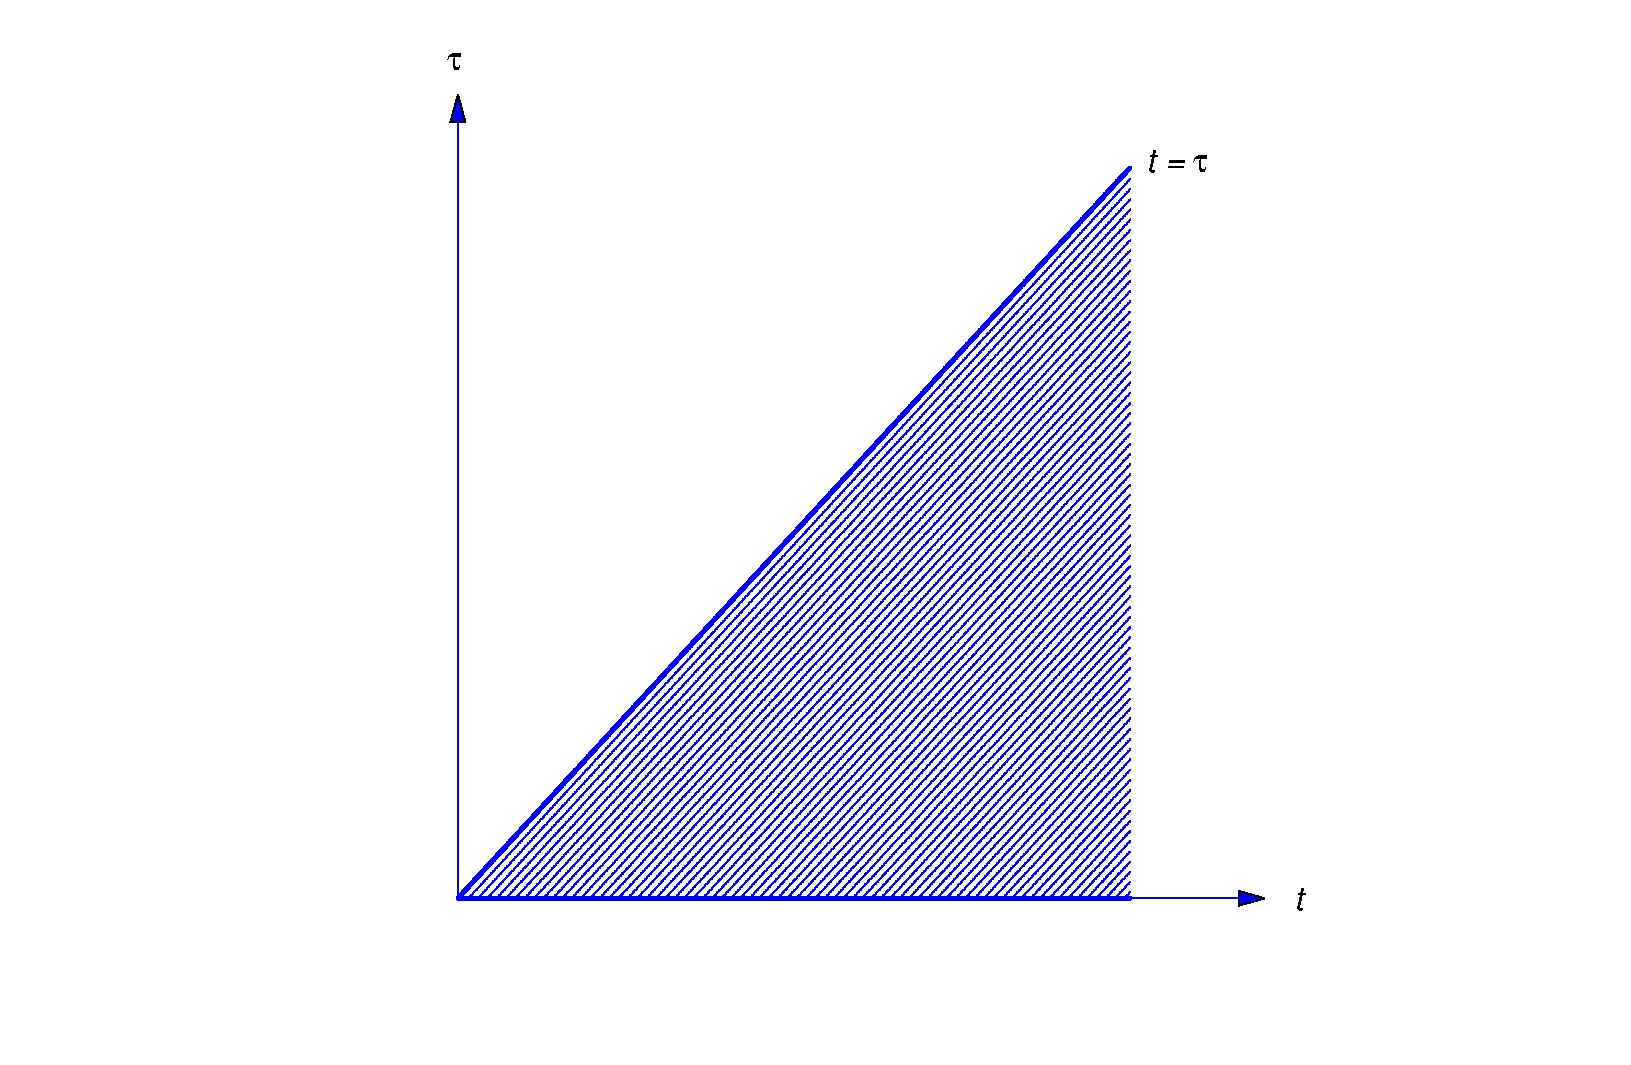
\includegraphics[bb=-78 148 689 643, width=5.67in, height=3.66in, keepaspectratio]{fig080601}
  \caption{The region of integration for the convolution theorem}
  \label{figure:8.6.1}
\end{figure}

\begin{example}
  \label{example:8.6.1}\rm Let
  \[
    f(t)=e^{at}\mbox{\quad and \quad}g(t)=e^{bt}\qquad(a\ne b).
  \]
  Verify that ${\cal L}(f\ast g)={\cal L}(f){\cal L}(g)$, as implied by the convolution theorem.
\end{example}

\solution We first compute
\[
  \begin{array}{ccccc}
    (f\ast g)(t) & = & \dst\int_{0}^{t}e^{a\tau}e^{b(t-\tau)}\,d\tau         & = & \dst e^{bt}\int_{0}^{t}e^{(a-b)\tau}d\tau       \\[2\jot]
                 & = & \dst{e^{bt}\frac{e^{(a-b)\tau}}{a-b}\,\bigg|^{t}_{0}} & = & \dst\frac{e^{bt}\left[e^{(a-b)t}-1\right]}{a-b} \\[2\jot]
                 & = & \dst\frac{e^{at}-e^{bt}}{a-b}.
  \end{array}
\]
Since
\[
  e^{at}\leftrightarrow\frac{1}{s-a}\quad\mbox{ and }\quad e^{bt}\leftrightarrow\frac{1}{s-b},
\]
it follows that
\begin{eqnarray*}
  {\cal L}(f\ast g) & = & \frac{1}{a-b}\left[\frac{1}{s-a}-\frac{1}{s-b}\right] \\[10pt]
                    & = & \frac{1}{(s-a)(s-b)}                                  \\[2\jot]
                    & = & {\cal L}(e^{at}){\cal L}(e^{bt})={\cal L}(f){\cal L}(g).
\end{eqnarray*}

\boxit{A Formula for the Solution of an Initial Value Problem}

\noindent
The convolution theorem provides a formula for the solution of an initial value problem for a linear
constant coefficient second order equation with an unspecified forcing function. The next three examples illustrate
this.

\begin{example}
  \label{example:8.6.2}\rm Find a formula for the solution of the initial value problem
  \begin{equation}
    \label{eq:8.6.7}y''-2y'+y=f(t),\quad y(0)=k_{0},\quad y'(0)=k_{1}.
  \end{equation}
\end{example}

\solution Taking Laplace transforms in \eqref{eq:8.6.7} yields
\[
  (s^{2}-2s+1)Y(s)=F(s)+(k_{1}+k_{0}s)-2k_{0}.
\]
Therefore
\begin{eqnarray*}
  Y(s) & = & \frac{1}{(s-1)^{2}}F(s)+\frac{k_{1}+k_{0}s-2k_{0}}{(s-1)^{2}} \\[2\jot]
       & = & \frac{1}{(s-1)^{2}}F(s)+\frac{k_{0}}{s-1}+\frac{k_{1}-k_{0}}{(s-1)^{2}}.
\end{eqnarray*}
From the table of Laplace transforms,
\[
  {\cal L}^{-1}\left(\frac{k_{0}}{s-1}+\frac{k_{1}-k_{0}}{(s-1)^{2}}\right) =e^{t}\left(k_{0}+(k_{1}-k_{0})t\right).
\]
Since
\[
  \frac{1}{(s-1)^{2}}\leftrightarrow te^{t}\mbox{\quad and \quad }F(s) \leftrightarrow f(t),
\]
the convolution theorem implies that
\[
  {\cal L}^{-1}\left(\frac{1}{(s-1)^{2}}F(s)\right)= \int_{0}^{t}\tau e^{\tau}f(t-\tau)\,d\tau.
\]
Therefore the solution of \eqref{eq:8.6.7} is
\[
  y(t)=e^{t}\left(k_{0}+(k_{1}-k_{0})t\right)+\int_{0}^{t}\tau e^{\tau}f(t-\tau)\, d\tau.
\]

\begin{example}
  \label{example:8.6.3}\rm Find a formula for the solution of the initial value problem
  \begin{equation}
    \label{eq:8.6.8}y''+4y=f(t),\quad y(0)=k_{0},\quad y'(0)=k_{1}.
  \end{equation}
\end{example}

\solution Taking Laplace transforms in \eqref{eq:8.6.8} yields
\[
  (s^{2}+4)Y(s)=F(s)+k_{1}+k_{0}s.
\]
Therefore
\[
  Y(s)=\frac{1}{(s^{2}+4)}F(s)+\frac{k_{1}+k_{0}s}{s^{2}+4}.
\]
From the table of Laplace transforms,
\[
  {\cal L}^{-1}\left(\frac{k_{1}+k_{0}s}{s^{2}+4}\right)=k_{0}\cos2t+\frac{k_{1}}{2}\sin2t.
\]
Since
\[
  \frac{1}{(s^{2}+4)}\leftrightarrow\frac{1}{2}\sin2t\mbox{\quad and \quad}F(s)\leftrightarrow f(t),
\]
the convolution theorem implies that
\[
  {\cal L}^{-1}\left(\frac{1}{(s^{2}+4)}F(s)\right)= \frac{1}{2}\int_{0}^{t}f(t-\tau)\sin2\tau\, d\tau.
\]
Therefore the solution of \eqref{eq:8.6.8} is
\[
  y(t)=k_{0}\cos2t+\frac{k_{1}}{2}\sin2t+\frac{1}{2}\int_{0}^{t}f(t-\tau)\sin 2\tau\,d\tau.
\]

\begin{example}
  \label{example:8.6.4}\rm Find a formula for the solution of the initial value problem
  \begin{equation}
    \label{eq:8.6.9}y''+2y'+2y=f(t),\quad y(0)=k_{0},\quad y'(0)=k_{1}.
  \end{equation}
\end{example}

\solution Taking Laplace transforms in \eqref{eq:8.6.9} yields
\[
  (s^{2}+2s+2)Y(s)=F(s)+k_{1}+k_{0}s+2k_{0}.
\]
Therefore
\begin{eqnarray*}
  Y(s) & = & \frac{1}{(s+1)^{2}+1}F(s)+\frac{k_{1}+k_{0}s+2k_{0}}{(s+1)^{2}+1} \\[2\jot]
       & = & \frac{1}{(s+1)^{2}+1}F(s)+\frac{(k_{1}+k_{0})+k_{0}(s+1)}{(s+1)^{2}+1}.
\end{eqnarray*}
From the table of Laplace transforms,
\[
  {\cal L}^{-1}\left(\frac{(k_{1}+k_{0})+k_{0}(s+1)}{(s+1)^{2}+1}\right)= e^{-t}\left((k_{1}+k_{0})\sin t+k_{0}\cos t\right).
\]
Since
\[
  \frac{1}{(s+1)^{2}+1}\leftrightarrow e^{-t}\sin t\mbox{\quad and \quad}F(s)\leftrightarrow f(t),
\]
the convolution theorem implies that
\[
  {\cal L}^{-1}\left(\frac{1}{(s+1)^{2}+1}F(s)\right)= \int_{0}^{t}f(t-\tau)e^{-\tau}\sin\tau \,d\tau.
\]
Therefore the solution of \eqref{eq:8.6.9} is
\begin{equation}
  \label{eq:8.6.10}y(t)=e^{-t}\left((k_{1}+k_{0})\sin t+k_{0}\cos t\right)+\int_{0}^{t}f(t-\tau)e^{-\tau}\sin\tau\,d\tau.
\end{equation}

\boxit{Evaluating Convolution Integrals}

\noindent
We'll say that an integral of the form $\int_{0}^{t}u(\tau)v(t-\tau)\,d\tau$ is a {\color{blue}\it
convolution integral\/}. The convolution theorem provides a convenient way to evaluate convolution
integrals.

\begin{example}
  \label{example:8.6.5}\rm Evaluate the convolution integral
  \[
    h(t)=\int_{0}^{t}(t-\tau)^{5}\tau^{7}d\tau.
  \]
\end{example}

\solution We could evaluate this integral by expanding $(t-\tau)^{5}$ in powers of $\tau$ and then
integrating. However, the convolution theorem provides an easier way. The integral is the
convolution of $f(t)=t^{5}$ and $g(t)=t^{7}$. Since
\[
  t^{5}\leftrightarrow\frac{5!}{s^{6}}\quad\mbox{ and }\quad t^{7}\leftrightarrow\frac{7!}{s^{8}},
\]
the convolution theorem implies that
\[
  h(t)\leftrightarrow\frac{5!7!}{s^{14}}=\frac{5!7!}{13!}\,\frac{13!}{s^{14}},
\]
where we have written the second equality because
\[
  \frac{13!}{s^{14}}\leftrightarrow t^{13}.
\]
Hence,
\[
  h(t)=\frac{5!7!}{13!}\,t^{13}.
\]

\begin{example}
  \label{example:8.6.6}\rm Use the convolution theorem and a partial fraction expansion to evaluate
  the convolution integral
  \[
    h(t)=\int_{0}^{t}\sin a(t-\tau)\cos b\tau\,d\tau\quad(|a|\ne|b|).
  \]
\end{example}

\solution Since
\[
  \sin at\leftrightarrow\frac{a}{s^{2}+a^{2}}\quad\mbox{and}\quad \cos bt\leftrightarrow\frac{s}{s^{2}+b^{2}},
\]
the convolution theorem implies that
\[
  H(s)=\frac{a}{s^{2}+a^{2}}\frac{s}{s^{2}+b^{2}}.
\]
Expanding this in a partial fraction expansion yields
\[
  H(s)=\frac{a}{b^{2}-a^{2}}\left[\frac{s}{s^{2}+a^{2}}-\frac{s}{s^{2}+b^{2}}\right].
\]
Therefore
\[
  h(t)=\frac{a}{b^{2}-a^{2}}\left(\cos at-\cos bt\right).
\]

\boxit{Volterra Integral Equations}

\noindent
An equation of the form
\begin{equation}
  \label{eq:8.6.11}y(t)=f(t)+\int_{0}^{t}k(t-\tau)y(\tau)\,d\tau
\end{equation}
is a
\href{https://mathshistory.st-andrews.ac.uk/Biographies/Volterra/}{\color{blue}
\it Volterra integral equation}. Here $f$ and $k$ are given functions and $y$ is unknown. Since the
integral on the right is a convolution integral, the convolution theorem provides a convenient
formula for solving \eqref{eq:8.6.11}. Taking Laplace transforms in \eqref{eq:8.6.11} yields
\[
  Y(s)=F(s)+K(s)Y(s),
\]
and solving this for $Y(s)$ yields
\[
  Y(s)=\frac{F(s)}{1-K(s)}.
\]
We then obtain the solution of \eqref{eq:8.6.11} as $y={\cal L}^{-1}(Y)$.

\begin{example}
  \label{example:8.6.7}\rm Solve the integral equation
  \begin{equation}
    \label{eq:8.6.12}y(t)=1+2\int_{0}^{t}e^{-2(t-\tau)}y(\tau)\,d\tau.
  \end{equation}
\end{example}

\solution Taking Laplace transforms in \eqref{eq:8.6.12} yields
\[
  Y(s)=\frac{1}{s}+\frac{2}{s+2}Y(s),
\]
and solving this for $Y(s)$ yields
\[
  Y(s)=\frac{1}{s}+\frac{2}{s^{2}}.
\]
Hence,
\[
  y(t)=1+2t.
\]

\boxit{Transfer Functions}

\noindent
The next theorem presents a formula for the solution of the general initial value problem
\[
  ay''+by'+cy=f(t),\quad y(0)=k_{0},\quad y'(0)=k_{1},
\]
where we assume for simplicity that $f$ is continuous on $[0,\infty)$ and that ${\cal L}(f)$ exists.
In Exercises~\ref{exer:8.6.11}--\ref{exer:8.6.14} it's shown that the formula is valid under much
weaker conditions on $f$.

\begin{theorem}
  \color{blue}
  \label{thmtype:8.6.3} Suppose $f$ is continuous on $[0,\infty)$ and has a Laplace transform. Then
  the solution of the initial value problem
  \begin{equation}
    \label{eq:8.6.13}ay''+by'+cy=f(t),\quad y(0)=k_{0},\quad y'(0)=k_{1},
  \end{equation}
  is
  \begin{equation}
    \label{eq:8.6.14}y(t)=k_{0}y_{1}(t)+k_{1}y_{2}(t)+\int_{0}^{t}w(\tau)f(t-\tau)\,d\tau,
  \end{equation}
  where $y_{1}$ and $y_{2}$ satisfy
  \begin{equation}
    \label{eq:8.6.15}ay_{1}''+by_{1}'+cy_{1}=0,\quad y_{1}(0)=1,\quad y_{1}'(0)=0,
  \end{equation}
  and
  \begin{equation}
    \label{eq:8.6.16}ay_{2}''+by_{2}'+cy_{2}=0,\quad y_{2}(0)=0,\quad y_{2}'(0)=1,
  \end{equation}
  and
  \begin{equation}
    \label{eq:8.6.17}w(t)=\frac{1}{a}y_{2}(t).
  \end{equation}
\end{theorem}

\proof Taking Laplace transforms in \eqref{eq:8.6.13} yields
\[
  p(s)Y(s)=F(s)+a(k_{1}+k_{0}s)+bk_{0},
\]
where
\[
  p(s)=as^{2}+bs+c.
\]
Hence,
\begin{equation}
  \label{eq:8.6.18}Y(s)=W(s)F(s)+V(s)
\end{equation}
with
\begin{equation}
  \label{eq:8.6.19}W(s)=\frac{1}{p(s)}
\end{equation}
and
\begin{equation}
  \label{eq:8.6.20}V(s)=\frac{a(k_{1}+k_{0}s)+bk_{0}}{p(s)}.
\end{equation}

Taking Laplace transforms in \eqref{eq:8.6.15} and \eqref{eq:8.6.16} shows that
\[
  p(s)Y_{1}(s)=as+b\quad\mbox{and}\quad p(s)Y_{2}(s)=a.
\]
Therefore
\[
  Y_{1}(s)=\frac{as+b}{p(s)}
\]
and
\begin{equation}
  \label{eq:8.6.21}Y_{2}(s)=\frac{a}{p(s)}.
\end{equation}
Hence, \eqref{eq:8.6.20} can be rewritten as
\[
  V(s)=k_{0}Y_{1}(s)+k_{1}Y_{2}(s).
\]
Substituting this into \eqref{eq:8.6.18} yields
\[
  Y(s)=k_{0}Y_{1}(s)+k_{1}Y_{2}(s)+\frac{1}{a}Y_{2}(s)F(s).
\]
Taking inverse transforms and invoking the convolution theorem yields \eqref{eq:8.6.14}. Finally,
\eqref{eq:8.6.19} and \eqref{eq:8.6.21} imply \eqref{eq:8.6.17}.\bbox

It is useful to note from \eqref{eq:8.6.14} that $y$ is of the form
\[
  y=v+h,
\]
where
\[
  v(t)=k_{0}y_{1}(t)+k_{1}y_{2}(t)
\]
depends on the initial conditions and is independent of the forcing function, while
\[
  h(t)=\int_{0}^{t}w(\tau)f(t-\tau)\, d\tau
\]
depends on the forcing function and is independent of the initial conditions. If the zeros of the
characteristic polynomial
\[
  p(s)=as^{2}+bs+c
\]
of the complementary equation have negative real parts, then $y_{1}$ and $y_{2}$ both approach zero
as $t\to\infty$, so $\lim_{t\to\infty}v(t)=0$ for any choice of initial conditions. Moreover, the
value of $h(t)$ is essentially independent of the values of $f(t-\tau)$ for large $\tau$, since
$\lim_{\tau\to\infty}w(\tau)=0$. In this case we say that $v$ and $h$ are {\color{blue}\it
transient\/} and {\color{blue}\it steady state components\/}, respectively, of the solution $y$ of
\eqref{eq:8.6.13}. These definitions apply to the initial value problem of
Example~\ref{example:8.6.4}, where the zeros of
\[
  p(s)=s^{2}+2s+2=(s+1)^{2}+1
\]
are $-1\pm i$. From \eqref{eq:8.6.10}, we see that the solution of the general initial value problem
of Example~\ref{example:8.6.4} is $y=v+h$, where
\[
  v(t)=e^{-t}\left((k_{1}+k_{0})\sin t+k_{0}\cos t\right)
\]
is the transient component of the solution and
\[
  h(t)=\int_{0}^{t}f(t-\tau)e^{-\tau}\sin\tau\,d\tau
\]
is the steady state component. The definitions don't apply to the initial value problems considered
in Examples~\ref{example:8.6.2} and \ref{example:8.6.3}, since the zeros of the characteristic
polynomials in these two examples don't have negative real parts.

In physical applications where the input $f$ and the output $y$ of a device are related by
\eqref{eq:8.6.13}, the zeros of the characteristic polynomial usually do have negative real parts.
Then $W={\cal L}(w)$ is called the {\color{blue}\it transfer function\; } of the device. Since
\[
  H(s)=W(s)F(s),
\]
we see that
\[
  W(s)=\frac{H(s)}{F(s)}
\]
is the ratio of the transform of the steady state output to the transform of the input.

Because of the form of
\[
  h(t)=\int_{0}^{t}w(\tau)f(t-\tau)\,d\tau,
\]
$w$ is sometimes called the {\color{blue}\it weighting function} of the device, since it assigns
weights to past values of the input $f$. It is also called the {\color{blue}\it impulse response} of
the device, for reasons discussed in the next section.

Formula \eqref{eq:8.6.14} is given in more detail in Exercises~\ref{exer:8.6.8}--\ref{exer:8.6.10}
for the three possible cases where the zeros of $p(s)$ are real and distinct, real and repeated, or
complex conjugates, respectively.

\exercises

\begin{exerciselist}
  \item\label{exer:8.6.1} Express the inverse transform as an integral.

  \begin{description}
    \item
      \begin{tabular}[t]{@{}p{168pt}@{}p{168pt}}
        \part{a} $\dst\frac{1}{s^{2}(s^{2}+4)}$ & \part{b} $\dst\frac{s}{(s+2)(s^{2}+9)}$
      \end{tabular}

    \item
      \begin{tabular}[t]{@{}p{168pt}@{}p{168pt}}
        \part{c} $\dst\frac{s}{(s^{2}+4)(s^{2}+9)}$ & \part{d} $\dst\frac{s}{(s^{2}+1)^{2}}$
      \end{tabular}

    \item
      \begin{tabular}[t]{@{}p{168pt}@{}p{168pt}}
        \part{e} $\dst\frac{1}{s(s-a)}$ & \part{f} $\dst\frac{1}{(s+1)(s^{2}+2s+2)}$
      \end{tabular}

    \item
      \begin{tabular}[t]{@{}p{168pt}@{}p{168pt}}
        \part{g} $\dst\frac{1}{(s+1)^{2}(s^{2}+4s+5)}$ & \part{h} $\dst\frac{1}{(s-1)^{3}(s+2)^{2}}$
      \end{tabular}

    \item
      \begin{tabular}[t]{@{}p{168pt}@{}p{168pt}}
        \part{i} $\dst\frac{s-1}{s^{2}(s^{2}-2s+2)}$ & \part{j} $\dst\frac{s(s+3)}{(s^{2}+4)(s^{2}+6s+10)}$
      \end{tabular}

    \item
      \begin{tabular}[t]{@{}p{168pt}@{}p{168pt}}
        \part{k} $\dst\frac{1}{(s-3)^{5}s^{6}}$ & \part{l} $\dst\frac{1}{(s-1)^{3}(s^{2}+4)}$
      \end{tabular}

    \item
      \begin{tabular}[t]{@{}p{168pt}@{}p{168pt}}
        \part{m} $\dst\frac{1}{s^{2}(s-2)^{3}}$ & \part{n} $\dst\frac{1}{s^{7}(s-2)^{6}}$
      \end{tabular}
  \end{description}

  \item\label{exer:8.6.2} Find the Laplace transform.

  \begin{description}
    \item
      \begin{tabular}[t]{@{}p{168pt}@{}p{168pt}}
        \part{a} $\dst{\int_{0}^{t}\sin a\tau\cos b(t-\tau)\,d\tau}$ & \part{b} $\dst{\int_{0}^{t}e^{\tau}\sin a(t-\tau)\,d\tau}$
      \end{tabular}

    \item
      \begin{tabular}[t]{@{}p{168pt}@{}p{168pt}}
        \part{c} $\dst{\int_{0}^{t}\sinh a\tau\cosh a(t-\tau)\,d\tau}$ & \part{d} $\dst{\int_{0}^{t}\tau(t-\tau)\sin\omega\tau\cos\omega (t-\tau)\,d\tau}$
      \end{tabular}

    \item
      \begin{tabular}[t]{@{}p{168pt}@{}p{168pt}}
        \part{e} $\dst{e^{t}\int_{0}^{t}\sin\omega\tau \cos\omega(t-\tau)\,d\tau}$ & \part{f} $\dst{e^{t}\int_{0}^{t}\tau^{2}(t-\tau)e^{\tau}\,d\tau}$
      \end{tabular}

    \item
      \begin{tabular}[t]{@{}p{168pt}@{}p{168pt}}
        \part{g} $\dst{e^{-t}\int_{0}^{t}e^{-\tau}\tau\cos\omega(t-\tau)\,d\tau}$ & \part{h} $\dst{e^{t}\int_{0}^{t}e^{2\tau}\sinh (t-\tau)\,d\tau}$
      \end{tabular}

    \item
      \begin{tabular}[t]{@{}p{168pt}@{}p{168pt}}
        \part{i} $\dst{\int_{0}^{t}\tau e^{2\tau}\sin 2(t-\tau)\,d\tau}$ & \part{j} $\dst{\int_{0}^{t}(t-\tau)^{3}e^{\tau}\,d\tau}$
      \end{tabular}

    \item
      \begin{tabular}[t]{@{}p{168pt}@{}p{168pt}}
        \part{k} $\dst{\int_{0}^{t}\tau^{6} e^{-(t-\tau)}\sin3(t-\tau)\,d\tau}$ & \part{l} $\dst{\int_{0}^{t}\tau^{2}(t-\tau)^{3}\, d\tau}$
      \end{tabular}

    \item
      \begin{tabular}[t]{@{}p{168pt}@{}p{168pt}}
        \part{m} $\dst{\int_{0}^{t}(t-\tau)^{7}e^{-\tau} \sin2\tau\,d\tau}$ & \part{n} $\dst{\int_{0}^{t}(t-\tau)^{4}\sin 2\tau\,d\tau}$
      \end{tabular}
  \end{description}

  \item\label{exer:8.6.3} Find a formula for the solution of the initial value problem.

  \begin{description}
    \item \part{a} $y''+3y'+y=f(t),\quad y(0)=0,\quad y'(0)=0$

    \item \part{b} $y''+4y=f(t),\quad y(0)=0,\quad y'(0)=0$

    \item \part{c} $y''+2y'+y=f(t),\quad y(0)=0,\quad y'(0)=0$

    \item \part{d} $y''+k^{2}y=f(t),\quad y(0)=1,\quad y'(0)=-1$

    \item \part{e} $y''+6y'+9y=f(t),\quad y(0)=0,\quad y'(0)=-2$

    \item \part{f} $y''-4y=f(t),\quad y(0)=0,\quad y'(0)=3$

    \item \part{g} $y''-5y'+6y=f(t),\quad y(0)=1,\quad y'(0)=3$

    \item \part{h} $y''+\omega^{2}y=f(t),\quad y(0)=k_{0},\quad y'(0)=k_{1}$
  \end{description}

  \item\label{exer:8.6.4} Solve the integral equation.

  \begin{description}
    \item \part{a} $\dst{y(t)=t-\int_{0}^{t}(t-\tau) y(\tau)\,d\tau}$

    \item \part{b} $\dst{y(t)=\sin t-2 \int_{0}^{t}\cos(t-\tau)y(\tau)\,d\tau}$

    \item
      \begin{tabular}[t]{@{}p{168pt}@{}p{168pt}}
        \part{c} $\dst{y(t)=1+2 \int_{0}^{t}y(\tau)\cos(t-\tau)\,d\tau}$ & \part{d} $\dst{y(t)=t+\int_{0}^{t} y(\tau)e^{-(t-\tau)}\,d\tau}$
      \end{tabular}

    \item \part{e} $\dst{y'(t)=t+\int_{0}^{t}y(\tau)\cos (t-\tau)\,d\tau,\,y(0)=4}$

    \item \part{f} $\dst{y(t)=\cos t-\sin t+ \int_{0}^{t}y(\tau)\sin(t-\tau)\,d\tau}$\\[2\jot]
  \end{description}

  \item\label{exer:8.6.5} Use the convolution theorem to evaluate the integral.

  \begin{description}
    \item
      \begin{tabular}[t]{@{}p{168pt}@{}p{168pt}}
        \part{a} $\dst{\int_{0}^{t}(t-\tau)^{7}\tau^{8}\, d\tau}$ & \part{b} $\dst{\int_{0}^{t}(t-\tau)^{13}\tau^{7}\,d\tau}$
      \end{tabular}

    \item
      \begin{tabular}[t]{@{}p{168pt}@{}p{168pt}}
        \part{c} $\dst{\int_{0}^{t}(t-\tau)^{6}\tau^{7}\, d\tau}$ & \part{d} $\dst{\int_{0}^{t}e^{-\tau}\sin(t-\tau)\,d\tau}$
      \end{tabular}

    \item \part{e} $\dst{\int_{0}^{t}\sin\tau\cos2(t-\tau)\,d\tau}$\\[2\jot]
  \end{description}

  \item\label{exer:8.6.6} Show that
  \[
    \int_{0}^{t}f(t-\tau)g(\tau)\,d\tau=\int_{0}^{t}f(\tau)g(t-\tau)\,d\tau
  \]
  by introducing the new variable of integration $x=t-\tau$ in the first integral.

  \item\label{exer:8.6.7} Use the convolution theorem to show that if $f(t)\leftrightarrow F(s)$
        then
  \[
    \int_{0}^{t}f(\tau)\,d\tau\leftrightarrow\frac{F(s)}{s}.
  \]

  \item\label{exer:8.6.8} Show that if $p(s)=as^{2}+bs+c$ has distinct real zeros $r_{1}$ and
        $r_{2}$ then the solution of
  \[
    ay''+by'+cy=f(t),\quad y(0)=k_{0},\quad y'(0)=k_{1}
  \]
  is
  \begin{eqnarray*}
    y(t) & = & \;k_{0}\frac{r_{2}e^{r_{1}t}-r_{1}e^{r_{2}t}}{r_{2}-r_{1}}+k_{1}\frac{e^{r_{2}t}-e^{r_{1}t}}{r_{2}-r_{1}} \\
         &   & +\frac{1}{a(r_{2}-r_{1})}\int_{0}^{t}(e^{r_{2}\tau}-e^{r_{1}\tau})f(t-\tau)\,d\tau.
  \end{eqnarray*}

  \item\label{exer:8.6.9} Show that if $p(s)=as^{2}+bs+c$ has a repeated real zero $r_{1}$ then the
        solution of
  \[
    ay''+by'+cy=f(t),\quad y(0)=k_{0},\quad y'(0)=k_{1}
  \]
  is
  \[
    y(t)=\;k_{0}(1-r_{1}t)e^{r_{1}t}+k_{1}te^{r_{1}t}+\frac{1}{a}\int_{0}^{t}\tau e^{r_{1}\tau}f(t-\tau)\,d\tau.
  \]

  \item\label{exer:8.6.10} Show that if $p(s)=as^{2}+bs+c$ has complex conjugate zeros
        $\lambda\pm i\omega$ then the solution of
  \[
    ay''+by'+cy=f(t),\quad y(0)=k_{0},\quad y'(0)=k_{1}
  \]
  is
  \begin{eqnarray*}
    y(t) & = & \;e^{\lambda t}\left[k_{0}(\cos\omega t-\frac{\lambda}{\omega}\sin\omega t)+\frac{k_{1}}{\omega}\sin\omega t\right] \\
         &   & +\frac{1}{a\omega}\int_{0}^{t}e^{\lambda \tau}f(t-\tau)\sin\omega\tau\,d\tau.
  \end{eqnarray*}

  \item\label{exer:8.6.11} Let
  \[
    w={\cal L}^{-1}\left(\frac{1}{as^{2}+bs+c}\right),
  \]
  where $a$, $b$, and $c$ are constants and $a\ne0$.
  \begin{alist}
    \item % (a)
    Show that $w$ is the solution of
    \[
      aw''+bw'+cw=0,\quad w(0)=0,\quad w'(0)=\frac{1}{a}.
    \]

    \item % (b)
    Let $f$ be continuous on $[0,\infty)$ and define
    \[
      h(t)=\int_{0}^{t}w(t-\tau)f(\tau)\,d\tau.
    \]
    Use \href{https://mathshistory.st-andrews.ac.uk/Biographies/Leibniz/}{\color{blue}
    \it Leibniz's rule} for differentiating an integral with respect to a parameter to show that $h$
    is the solution of
    \[
      ah''+bh'+ch=f,\quad h(0)=0,\quad h'(0)=0.
    \]

    \item % (c)
    Show that the function $y$ in Eqn.~\eqref{eq:8.6.14} is the solution of Eqn.~\eqref{eq:8.6.13}
    provided that $f$ is continuous on $[0,\infty)$; thus, it's not necessary to assume that $f$ has
    a Laplace transform.
  \end{alist}

  \item\label{exer:8.6.12} Consider the initial value problem
  \[
    ay''+by'+cy=f(t),\quad y(0)=0,\quad y'(0)=0, \eqno{\rm(A)}
  \]
  where $a$, $b$, and $c$ are constants, $a\ne0$, and
  \[
    f(t)=\left\{
    \begin{array}{cc}
      f_{0}(t), & 0\le t<t_{1}, \\[5pt]
      f_{1}(t), & t\ge t_{1}.
    \end{array}\right.
  \]
  Assume that $f_{0}$ is continuous and of exponential order on $[0,\infty)$ and $f_{1}$ is
  continuous and of exponential order on $[t_{1},\infty)$. Let
  \[
    p(s)=as^{2}+bs+c.
  \]
  \begin{alist}
    \item % (a)
    Show that the Laplace transform of the solution of (A) is
    \[
      Y(s)=\frac{F_{0}(s)+e^{-st_{1}}G(s)}{p(s)}
    \]
    where $g(t)=f_{1}(t+t_{1})-f_{0}(t+t_{1})$.

    \item % (b)
    Let $w$ be as in Exercise~\ref{exer:8.6.11}. Use Theorem~\ref{thmtype:8.4.2} and the convolution
    theorem to show that the solution of (A) is
    \[
      y(t)=\int_{0}^{t}w(t-\tau)f_{0}(\tau)\,d\tau+u(t-t_{1})\int_{0}^{t-t_{1}}w(t-t_{1}-\tau)g(\tau)\,d\tau
    \]
    for $t>0$.

    \item % (c)
    Henceforth, assume only that $f_{0}$ is continuous on $[0,\infty)$ and $f_{1}$ is continuous on
    $[t_{1},\infty)$. Use Exercise~\ref{exer:8.6.11} \part{a} and \part{b} to show that
    \[
      y'(t)=\int_{0}^{t}w'(t-\tau)f_{0}(\tau)\,d\tau+u(t-t_{1})\int_{0}^{t-t_{1}}w'(t-t_{1}-\tau)g(\tau)\,d\tau
    \]
    for $t>0$, and
    \[
      y''(t)=\frac{f(t)}{a}+\int_{0}^{t}w''(t-\tau)f_{0}(\tau)\,d\tau+u(t-t_{1})\int_{0}^{t-t_{1}}w''(t-t_{1}-\tau)g(\tau)\,d\tau
    \]
    for $0<t<t_{1}$ and $t>t_{1}$. Also, show $y$ satisfies the differential equation in (A)
    on$(0,t_{1})$ and $(t_{1},\infty)$.

    \item % (d)
    Show that $y$ and $y'$ are continuous on $[0,\infty)$.
  \end{alist}

  \item\label{exer:8.6.13} Suppose
  \[
    f(t)=\left\{
    \begin{array}{cl}
      f_{0}(t),   & 0\le t<t_{1},       \\[5pt]
      f_{1}(t),   & t_{1}\le t<t_{2},   \\
                  & \vdots              \\
      f_{k-1}(t), & t_{k-1}\le t<t_{k}, \\[5pt]
      f_{k}(t),   & t\ge t_{k},
    \end{array}\right.
  \]
  where $f_{m}$ is continuous on $[t_{m},\infty)$ for $m=0,\dots,k$ (let $t_{0}=0$), and define
  \[
    g_{m}(t)=f_{m}(t+t_{m})-f_{m-1}(t+t_{m}),\,m=1,\dots,k.
  \]
  Extend the results of Exercise~\ref{exer:8.6.12} to show that the solution of
  \[
    ay''+by'+cy=f(t),\quad y(0)=0,\quad y'(0)=0
  \]
  is
  \[
    y(t)=\int_{0}^{t}w(t-\tau)f_{0}(\tau)\,d\tau+\sum_{m=1}^{k}u(t-t_{m}) \int_{0}^{t-t_{m}}w(t-t_{m}-\tau)g_{m}(\tau)\,d\tau.
  \]

  \item\label{exer:8.6.14} Let $\{t_{m}\}_{m=0}^{\infty}$ be a sequence of points such that
        $t_{0}=0$, $t_{m+1}>t_{m}$, and $\lim_{m\to\infty}t_{m}=\infty$. For each nonnegative
        integer $m$ let $f_{m}$ be continuous on $[t_{m},\infty)$, and let $f$ be defined on
        $[0,\infty)$ by
  \[
    f(t)=f_{m}(t),\quad t_{m}\le t<t_{m+1}\quad m=0,1,2\dots.
  \]
  Let
  \[
    g_{m}(t)=f_{m}(t+t_{m})-f_{m-1}(t+t_{m}),\quad m=1,2,\dots.
  \]
  Extend the results of Exercise~\ref{exer:8.6.13} to show that the solution of
  \[
    ay''+by'+cy=f(t),\quad y(0)=0,\quad y'(0)=0
  \]
  is
  \[
    y(t)=\int_{0}^{t}w(t-\tau)f_{0}(\tau)\,d\tau+\sum_{m=1}^{\infty}u(t-t_{m}) \int_{0}^{t-t_{m}}w(t-t_{m}-\tau)g_{m}(\tau) \,d\tau.
  \]
  \hint{See Exercise{\ref{exer:8.4.30}.}}
\end{exerciselist}
